\section{Zupa krem z cukinii}
\bigskip
\small
\begin{minipage}{0.45\textwidth}
    \noindent \textbf{Czas:} 60 minut \\
    \textbf{Poziom trudności:} łatwy
\end{minipage}
\begin{minipage}{0.45\textwidth}
    \noindent \textbf{Ilość sprzątania:} średnia\\
    \textbf{Wymagany mysi sprzęt:} duży garnek, blender
\end{minipage}
\normalsize
\vspace{0.5cm}

\begin{multicols}{2}

\subsection*{Składniki}
\begin{itemize}
    \item 2 średniej wielkości marchewki
    \item 2 średniej wielkości korzenie pietruszki
    \item 1 cebula
    \item 6 dużych ząbków czosnku
    \item 4 duże cukinie
    \item 1 opakowanie śmietany 18\%
    \item ok. 100 g sera z niebieską pleśnią (np. Lazur, Grand Blue)
    \item oliwa do smażenia
    \item 1 łyżka masła
    \item przyprawy
    \item kostka rosołowa (opcjonalnie)
    \item sól i pieprz do smaku
\end{itemize}

\columnbreak

\begin{figure}[H]
    \centering
    \fbox{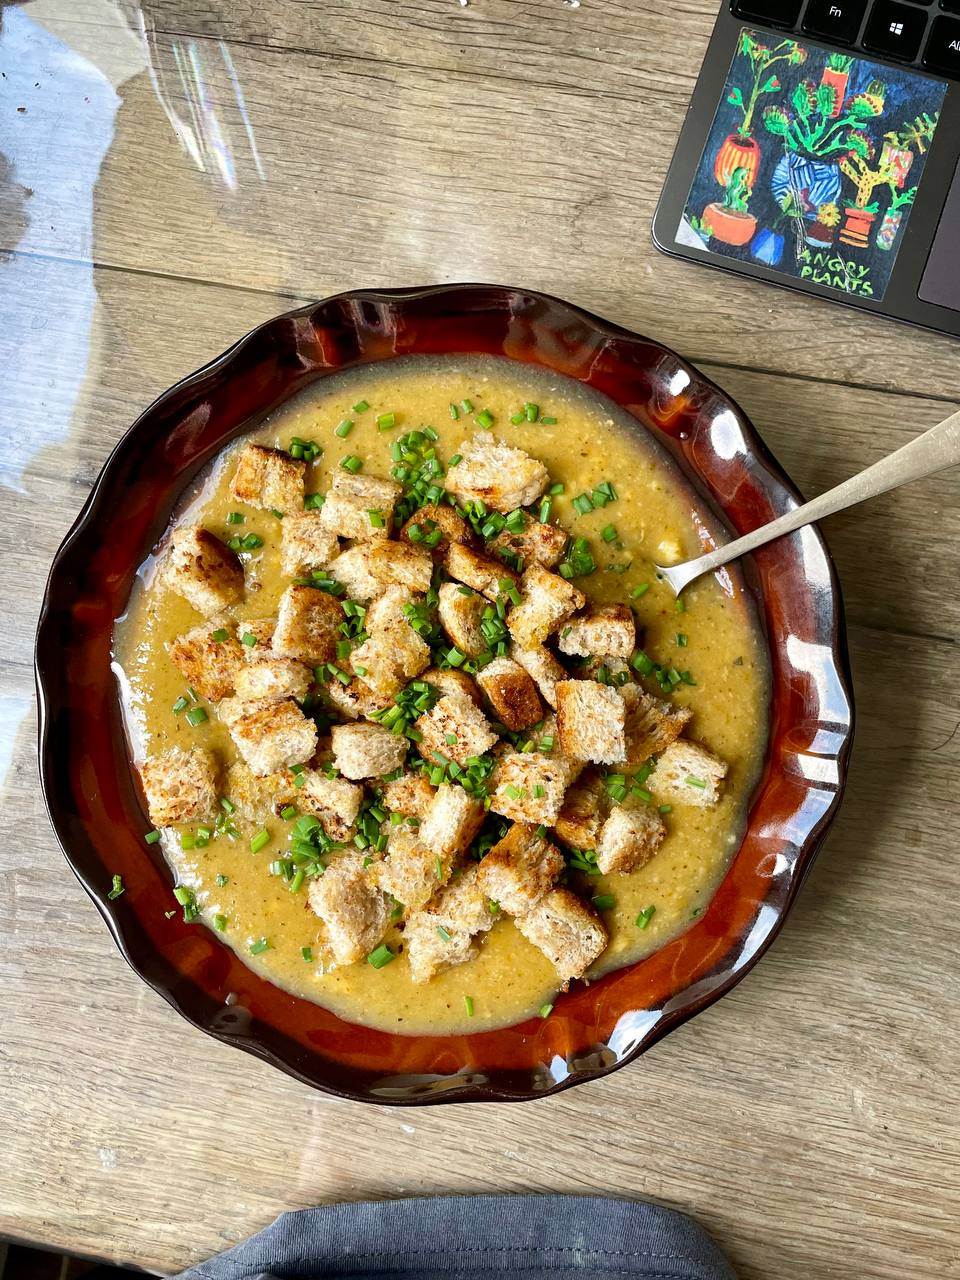
\includegraphics[width=0.4\textwidth]{images/zupa-cukiniowa.jpg}}
\end{figure}
\end{multicols}

\vspace{0.5cm}

\subsection*{Instruktaż}
\begin{enumerate}
    \item Cukinie dokładnie umyć i odkroić łodygę. Obieraczką do warzyw obierać każdą cukinię "w paski" , tzn. naprzemiennie na każdy obrany pasek pozostawić podobnej grubości pasek nieobranej skórki. Obrane cukinie przekroić wzdłuż na połowy, po czym każdą połowę przekroić ponownie wzdłuż. Jeśli pestek cukinii wewnątrz ćwiartek będzie zbyt wiele lub pojedyncze pestki będą łatwo widoczne, wyciąć nożem miąższ z nadmiarem pestek. Obrane i oczyszczone kawałki cukinii pokroić na duże kostki i odstawić na bok.
    \item Pietruszkę oraz marchew obrać, przekroić wzdłuż na pół i pokroić na kawałki, po czym podsmażać na rozgrzanej oliwie i średnim ogniu przez około 5 minut (lub aż się zarumienią) od czasu do czasu mieszając. Dodać łyżeczkę soli, aby warzywa puściły wodę. W międzyczasie pokroić cebulę na średniej wielkości kostkę (nie musi być dokładna) i obrać czosnek.
    \item Po zarumienieniu się pietruszki i marchewki dosypać cebulę i podsmażać mieszając do momentu, aż cebula się zeszkli, czyli również około 5 minut. Warzywa posypać płaską łyżeczką kolejno: pieprzu, bazylii, majeranku, tymianku, rozmarynu i ewentualnie rozgniecioną kostkę rosołową. Wszystko dokładnie wymieszać. Obniżyć ogień na niski, warzywa na dnie garnka przesunąć na bok tak, aby się nie przypaliły.
    \item W wydzielone miejsce dodać masło i przeciśnięty przez praskę czosnek stale mieszając go w maśle tak, aby się nie przypalił, czyli około 20 sekund aż stanie się wonny. Po upływie 20 sekund wszystkie warzywa dokładnie wymieszać.
    \item Do garnka dodać pokrojoną cukinię i dokładnie wymieszać z warzywami znajdującymi się na dnie garnka. Całość zalać taką ilością wrzątku, aby wszystkie warzywa były zanurzone. Dodać łyżeczkę soli, wymieszać i gotować pod przykryciem na małym ogniu od czasu do czasu mieszając przez co najmniej 45 minut, aczkolwiek im dłużej, tym lepiej.
    \item Po skończonym gotowaniu ostudzić lekko zupę (można wystawić garnek na balkon w chłodną pogodę) i zblendować dokładnie. Śmietanę rozrobić z 2-3 łyżkami gorącej zupy i wlać do garnka. Dosolić do smaku i w razie potrzeby, gdyby zupa była zbyt gęsta, dolać odrobinę wody, aby uzyskać pożądaną konsystencję.
\end{enumerate}

\vspace{0.5cm}

\small
\subsection*{Propozycja podania}
Z domowymi grzankami, z chrupiącym tostem, ze startym długodojrzewającym serem, ze świeżymi ziołami.

\vspace{0.3cm}

\subsection*{Dodatkowe uwagi}
Zupa świetnie się mrozi, dlatego też można bez problemu ugotować większą ilość, pozostawić do ostudzenia i przelać do pojemniczków, w których bezpiecznie się zamrozi - taki zapas awaryjny często przydaje się w dni, w które brakuje nam sił, aby ugotować obiad :)

\newpage
